\documentclass[11pt,a4paper]{article}

\usepackage[margin=0.8in]{geometry}
\usepackage[utf8]{inputenc}
\usepackage{amsmath}
\usepackage{amsfonts}
\usepackage{amssymb}
\usepackage[hidelinks]{hyperref}
\usepackage{float}

%% Bibliography/references packages
\usepackage[comma]{natbib}
%%\bibliographystyle{agsm}
\bibliographystyle{dcu}

%% Make bibliography show in table of contents
%% https://tex.stackexchange.com/questions/8458/making-the-bibliography-appear-in-the-table-of-contents
\usepackage[nottoc,numbib]{tocbibind}
%% ^^^ overwrites \bibname, so set it back
\renewcommand{\bibname}{References}

\RequirePackage{filecontents}
\begin{filecontents}{soft354_bib.bib}
@online{wikipedia:dft,
  author = {Wikipedia},
  title = {Discrete Fourier transform},
  year = 2018,
  url = {https://en.wikipedia.org/wiki/Discrete\_Fourier\_transform},
  urldate = {2018-01-15}
}
@online{server:gpu,
  author = {Amazon AWS},
  title = {Introducing Amazon EC2 P2 Instances, the largest GPU-Powered virtual machine in the cloud},
  year = 2018,
  url = {https://aws.amazon.com/about-aws/whats-new/2016/09/introducing-amazon-ec2-p2-instances-the-largest-gpu-powered-virtual-machine-in-the-cloud/},
  urldate = {2016-09-26}
}
@Book{fft_adv_dis,
author = {James S. Walker},
title = {Fast Fourier Transforms},
publisher = {CRC Press},
year = {1996},
OPTedition = {2}
}
@misc{arndt2002algorithms,
  title={Algorithms For Programmers},
  author={Arndt, J{\"o}rg},
  year = 2002
}

\end{filecontents}

%s comments
\usepackage{verbatim}

%inline graphs
\usepackage{wrapfig}
% multiple figures on line
\usepackage{subfig}

\usepackage{graphicx}
\graphicspath{ {img/} }

% Caption font size
% https://tex.stackexchange.com/questions/86120/font-size-of-figure-caption-header
\usepackage[font=scriptsize,labelfont=bf]{caption}

\setlength{\belowcaptionskip}{-10pt}
\setlength{\abovecaptionskip}{-5pt} % Chosen fairly arbitrarily


\usepackage{fancyhdr}
\pagestyle{fancy}
\lhead{\rightmark}
\chead{}
\rhead{SOFT354 - Parallel Computing and Distributed Systems}
\lfoot{\thepage}
\cfoot{}
\rfoot{Ben Lancaster 10424877}

\renewcommand{\subsectionmark}[1]{\markright{\thesubsection\ #1}}


\begin{document}

\begin{titlepage}
\begin{center}

\vspace*{3cm}
\Large
\textbf{SOFT354 - Parallel Computing and Distributed Systems}

\vspace{0.4cm}
\large
Design, implementation, and evaluation of parallel Discrete Fourier Transform algorithms using MPI and CUDA.
%%A comparison of the Discrete Fourier Transform algorithm implemented in CUDA and MPI.

\vspace{4cm}
\textbf{Ben Lancaster}\\
\today

\vspace{4cm}
\textbf{Abstract}\\
\small
The DFT algorithm is a widely used algorithm used heavy in digital signal processing applications that enables conversion of a time-based signal to a frequency-based signal. The algorithm has $O(n^2)$ complexity resulting in long computation times for large data sets. Introducing parallel concepts to this sequential algorithms, like dividing the input samples over multiple processes, and utilizing GPU hardware with CUDA, can greatly increase the performance. Results show that a performance increase of 5x to 10x can be seen on small to large datasets using both MPI and CUDA solutions. 


\end{center}

\end{titlepage}

\renewcommand*\contentsname{Table of Contents}
\tableofcontents
\newpage

\section{Introduction}
This report discusses the design, implementation, and evaluation of a parallel Discrete Fourier Transform (DFT) algorithm using CUDA and MPI.
In signal processing, DFTs are used to represent signals as a series of sinusoidal waveforms at different frequencies and amplitudes. This is useful when wanting to identify specific audio components in speed recognition. 

\begin{figure}[H]%
    \centering
    \subfloat[Time domain]{{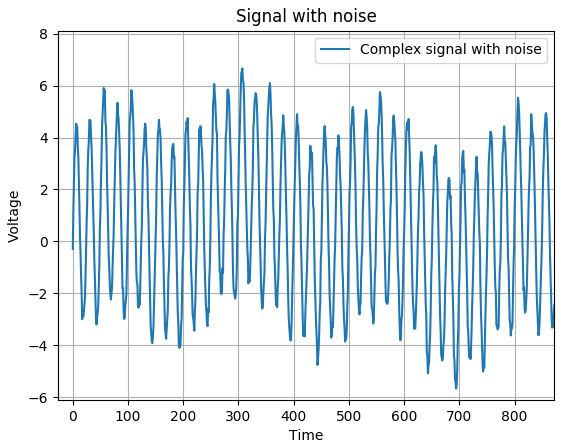
\includegraphics[width=7cm]{intro_signal} }}%
    \qquad
    \subfloat[Frequency domain]{{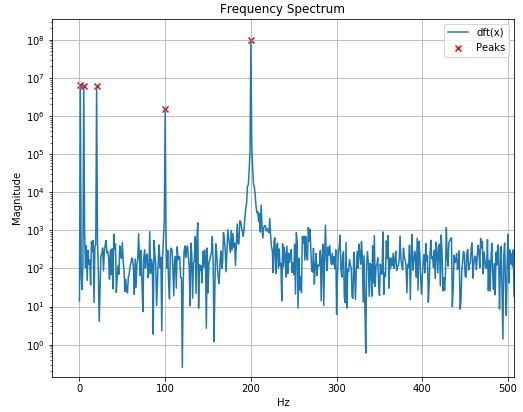
\includegraphics[width=7cm]{intro_dft} }}%
    \vspace{5pt}
    \caption{\textbf{Left:} A compound signal made up of 1, 5, 20, 100, and 200 Hz sine waves in the time domain. \textbf{Right:} Frequency domain representation showing high amplitude peaks for the 1, 5, 20, 100, and 200 Hz waveforms.}%
    \label{fig:dft_demo}%
\end{figure}

An example application of the DFT algorithm is shown above in Figure \ref{fig:dft_demo}. The complex, compound signal on the left shown in the time domain is represented in the frequency domain on the right.

The 1 dimensional Discrete Fourier Transform algorithm is show in Figure \ref{fig:dft_algorithm}. The algorithm in a complex vector and produces a complex vector of the same length in the frequency domain. The output sample $X_{k}$ is equal to the sum of all inputs multiplied by the exponential function $-i2$$\pi$$kn/N$, where $i$ is the square root of -1; $2$$\pi$ is 360 degrees; $k$ and $n$ are integer indexes to time and frequency domains, respectively; and $N$ is the number of samples in the signal.

\begin{figure}[H]
\begin{center}
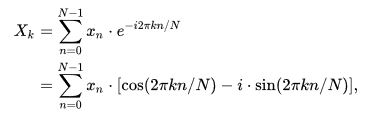
\includegraphics[scale=1]{dft_algorithm}
\end{center}
\caption{The Discrete Fourier Transform definition \citep{wikipedia:dft}.}
\label{fig:dft_algorithm}
\end{figure}

Using Euler's formula, we can rewrite the exponential function $e^{ix}$ to $cos x + i sin x$ which makes it easier to implement in code. This transformation is displayed in figure \ref{fig:dft_algorithm} (lower).

Each output sample must be calculated by acting upon all other samples in the input vector. This means the algorithm has a computation complexity of $O(n^2)$. A faster implementation of the DFT, called Fast Fourier Transform (FFT), achieves similar results in only $O(n\log(n))$ time. It achieves this by recursively dividing the input sample by 2 into separate \textit{bins}. The output of these bins can be reused, reducing the need to re-iterate over the input vector.

A disadvantage with FFT is that it requires the input vector length to be of a power of 2 \citep{fft_adv_dis}. If one wants to use FFT with a non-power-of-two length input, the input will need to need to be padded with 0's up to the next power of 2, or stripped down to the nearest. Padding with 0's has a negative impact on the output of the FFT function due to the FFT  working on 0Hz samples that will propagate through to other previous samples, offsetting their correct frequency output. If stripping down the input vector, information will be lost from the stripped samples.

Because of these disadvantages, a DFT function may be required instead, if output accuracy is favoured over speed. In this report, I will be designing, implementing, and evaluating, a parallel DFT algorithm using CUDA and MPI.

\section{Implementation}
This section discusses the design considerations and implementation of the parallel DFT algorithm in CUDA and MPI.

Both programs are run on a quad-core 4-thread Intel i5-4670k CPU at 4.3GHz with an NVIDIA GTX 970 GPU with 4GB memory, 1664 CUDA cores, 1050Mhz base clock, and featuring CUDA Compute Capability 5.2, which supports 1024 threads per block and 48KB maximum shared memory per block.

The software solution is split into 2 Visual Studio projects: soft354\_cuda and soft354\_mpi, for CUDA and MPI respectively. Only the CUDA and MPI libraries, and the \textit{windows.h} header (for time measurement, see later.) are required to build the two solutions. 
The CUDA solution is required to be built for the x64 architecture and the MPI solution is required to be built for the x86 architecture. The differences in the architectures will have a negligible effect on the performance of the programs. 

\begin{figure}[H]
\begin{center}
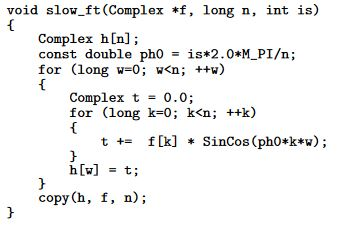
\includegraphics[scale=0.6]{code_dft_afp}
\end{center}
\caption{Code snipped of a Sequential DFT algorithm \citep{arndt2002algorithms}.}
\label{fig:code_dft_afp}
\end{figure}

Both of the parallel MPI and CUDA solutions I propose are based upon the sequential DFT algorithm proposed by Arndt \citep{arndt2002algorithms} but with parallel concepts applied to it.

\subsection{CUDA}

\begin{wrapfigure}{r}{0.4\textwidth}
\begin{center}
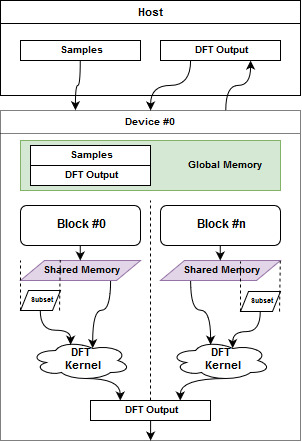
\includegraphics[scale=0.6]{cuda_impl1}
\end{center}
\caption{CUDA implementation control flow diagram showing memory }
\label{fig:cuda_impl1}
\end{wrapfigure}
The CUDA implementation utilises a host device, typically a CPU, to retrieve the input samples from a file and store the resulting output.   After reading the samples from a .csv file, the host allocates 2 global memory buffers on the device for the samples and output, and copies the input samples to the device.  Figure \ref{fig:cuda_impl1} displays the CUDA DFT algorithm's control flow.

Each thread is assigned a unique sample from the input vector. The thread then performs the DFT calculate using it's index, the samples value, and all other input sample points.

As the input samples are 1D dimensional, kernels are launched with a 1D grids and blocks to intuitively map threads to samples.
 The kernel assigns each output sample to a unique thread, identified by \textit{idx}. Each output sample must be calculated by iterating over the entire input sample vector. 

As the input sample size can contain many samples, the kernel will require many accesses to global memory. A technique, utilising the device's shared memory, is described in section \ref{sect:Dynamic Shared Memory} to reduce the number of global memory accesses.

Each thread writes it's result back into the global output buffer, which is then copied back from the device to the host.

\subsubsection{Dynamic Shared Memory} \label{sect:Dynamic Shared Memory}
As each operation on each sample requires values from all other samples, global memory accesses will be largest performance bottleneck. To reduce the amount of global memory accesses, I had the first thread of each block copy the complete global memory copy of the samples to a local shared memory buffer, which the DFT kernel would access instead of the global memory. Figure \ref{fig:code_cuda_all} shows the code segment that performs this process.

On Compute Capability 2.0 devices, the maximum shared memory size per block is 48KB, meaning that if the kernel was launched with 1 block, it could access all 48KB of memory. If two blocks were used, each block would have 24KB of memory available without delay.

\begin{figure}[H]%
    \centering
    \subfloat[CUDA kernel invocation showing amount of dynamic shared memory to allocate.]{{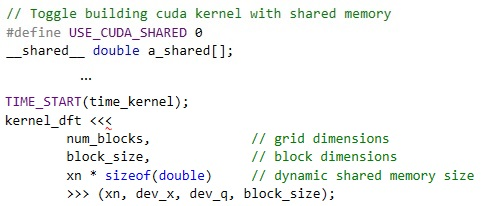
\includegraphics[width=7cm]{code_cuda} }}%
    \qquad
    \subfloat[First thread of each block copying all samples to the block's shared memory.]{{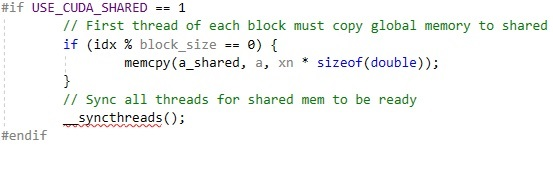
\includegraphics[width=8cm]{code_cuda_shared} }}%
    \vspace{5pt}
    \caption{}
    \label{fig:code_cuda_all}%
\end{figure}

To be able to fit the entire sample set in shared memory, I had to keep the maximum shared memory per block at it's highest by using as few blocks as possible. I used the maximum of 1024 threads per block for the GPU to reduce the number of required blocks.

Using any number of 8-byte samples below 2048, which would use up to 2 blocks of 1024 threads and 24KB of shared memory, allows all samples for each block to fit into their shared memory. 

\begin{wrapfigure}{r}{0.4\textwidth}
\begin{center}
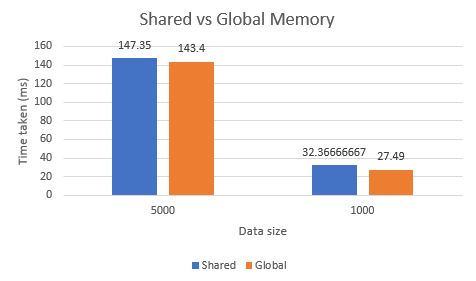
\includegraphics[scale=0.6]{shared_vs_global_graph}
\end{center}
\caption{Average kernel execution time using shared vs. global memory.}
\label{fig:shared_vs_global_graph}
\end{wrapfigure}

If using more than 2048 8-byte samples, resulting in using 3 or more blocks, results in the shared memory per block overflowing. The kernel handles this by pausing blocks that do not have enough shared memory ready, and running blocks that do have all their shared memory ready.

Even though we are accessing faster memory, it's size limitations causes resource availability delays when using larger data sets, which results in higher latency and lower performance. Figure \ref{fig:shared_vs_global_graph} shows the kernel execution time when using shared memory against global memory. We can see the global execution time is faster than shared memory. This is likely because the time taken for each block to copy the data set from global to shared memory (while other threads wait idle for the shared memory) is greater than the time of just accessing global memory.

%%\newpage
\subsection{MPI}
The MPI implementation is similar to the CUDA kernel. However, instead of each output sample being assigned to a unique thread, nodes are assigned a contiguous subset of the samples for which they perform the DFT function on, producing multiple outputs per node.

\begin{figure}[H]
\begin{center}
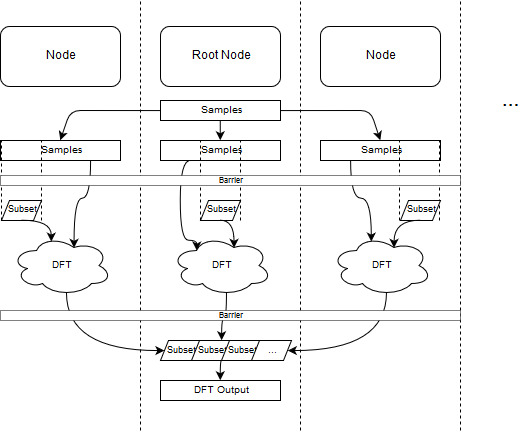
\includegraphics[scale=0.5]{mpi_impl1}
\end{center}
\caption{Control flow diagram of the parallel MPI DFT algorithm.}
\label{fig:mpi_impl1}
\end{figure}

The size of the subset of samples each node receives is calculated by dividing the total number of samples by the number of nodes. This distributes an equal number of samples to each node which allows each node to perform it's calculations and communications in similar time to the other nodes. This reduces the time spent by nodes being idle as they wait for other nodes to complete. The more MPI nodes used, the fewer samples allocated per node which reduces the number of DFT calculations required. Section \ref{sect:MPI Node Count} discusses the optimum node count and how to find it.

\begin{figure}[H]%
    \centering
    \subfloat[Contiguous sample subset assignment per MPI node code snippet. Located: main.c line 281.]{{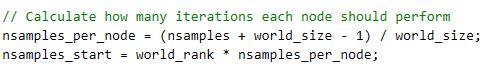
\includegraphics[width=7.5cm]{mpi_code_1} }}%
    \qquad
    \subfloat[Subset bounds checking for each MPI node. Located: main.c line 212.]{{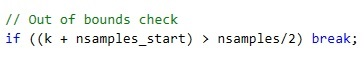
\includegraphics[width=6cm]{mpi_code_2} }}%
    \vspace{5pt}
    \caption{}%
    \label{fig:mpi_code}%
\end{figure}

Unlike the FFT algorithm, which only works for sample sizes equal to a power of 2, DFT works for any sample size. This means that the algorithm used to distribute the samples to each node will result in the last node to have an equal or less amount of samples than the other nodes. To account for this, the MPI DFT algorithm limits it's iterations to the number of samples. 

The MPI solution exploits the \textit{MPI\_Gather} feature of gathering from nodes in the order of their rank. This saves time re-ordering incoming output samples to match the input sample order.


\section{Evaluation}
\subsection{Measuring Performance}
Performance metrics have been captured using Windows' `\textit{QueryPerformanceCounter}` and the `NSight Performance Analysis` tools. Helper macros, `\textit{TIME\_START}` and `\textit{TIME\_STOP}` are used to record timed code sections.

Key performance metrics that have been analysed are: Memory allocation time, MPI broadcast and Gather time, MPI DFT calculation time, CUDA kernel execution time, CUDA memory operations time, CUDA kernel occupancy, and number of blocked CUDA warps.

Results shown in this report are averaged over multiple measurements to give a better estimate of real performance and reduce the effect of outliers. Raw measurements, which include repeat attempt timings, are found in the \textit{test/*.csv} directory.

As stated previously, all measurements were performed on a machine with a 4-core 4-thread Intel i5-4670k CPU at 4.3GHz with an NVIDIA GTX 970 GPU with 4GB memory, 1664 CUDA cores, 1050Mhz base clock, and featuring CUDA Compute Capability 5.2, which supports 1024 threads per block and 48KB maximum shared memory per block.

\subsection{MPI Node Count}\label{sect:MPI Node Count}
When running MPI on a single machine, MPI will spawn multiple nodes (processes) that are subject the OS's scheduling strategy. In addition, depending on available CPU resources, like core count, MPI and the OS will assign CPU resources to each processes.

\begin{wrapfigure}{r}{0.5\textwidth}
\begin{center}
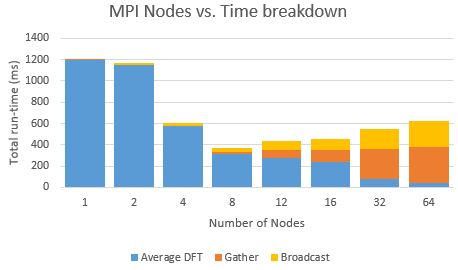
\includegraphics[scale=0.7]{mpi_eval_nodes}
\end{center}
\caption{Time breakdown of MPI program when run with different number of nodes.}
\label{fig:mpi_eval_nodes}
\end{wrapfigure}

Running on a 2 core, 4 thread CPU, with more MPI nodes than CPU threads, the OS will need to schedule each node with other running programs, which will reduce our MPI program's performance.

As seen in Figure \ref{fig:mpi_eval_nodes}, using fewer MPI nodes requires each node to work on more samples, which increases the average DFT calculate time. The small amount of nodes also means that little inter-process communication needs to take place to broadcast and gather the results. The \textit{Total run-time} metric starts when the MPI solution broadcasts the sample vector to each node, and ends after the gathering and combining of output samples. Therefore, this measurement includes all communication times as well as the DFT computation time.

Increasing the number of MPI nodes reduces the average DFT calculation time per node, as each node has fewer samples to work on, but inter-process communication is greatly increased. The MPI implementation uses blocking barrier communication messages to share and collect the results. With many nodes, it takes longer for MPI to synchronise the nodes resulting in longer total run-times.

From this, I predict that the optimum number of MPI nodes per machine for this algorithm is approximately 2x the total number of CPU threads.

\subsection{CUDA Threads Per Block}
Increasing the number of threads per block, whilst keeping the grid 1 dimensional, reduces the number of threads that need to write to shared memory. As discussed in \ref{sect:Dynamic Shared Memory}, the first node of each block copies the sample buffer from global memory to shared memory. This allows warps that would be waiting for shared memory to be ready, to become active and increase the occupancy of the kernel.

\begin{figure}[H]%
    \centering
    \subfloat[Time breakdown of CUDA program when run with different number of threads per block.]{{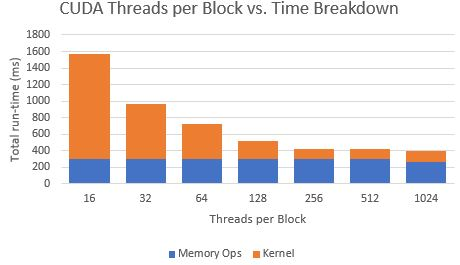
\includegraphics[width=7.5cm]{cuda_eval_threads} }}%
    \qquad
    \subfloat[Blocked Warps per block and Occupancy vs. Threads per Block.]{{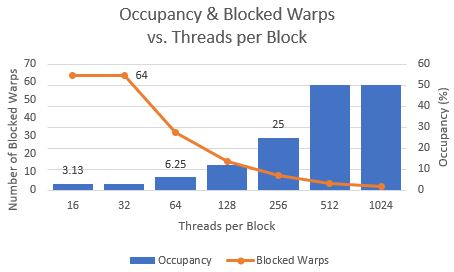
\includegraphics[width=7.5cm]{cuda_eval_occu} }}%
    \vspace{5pt}
    \caption{}%
    \label{fig:cuda_threads_per_block}%
\end{figure}

Figure \ref{fig:cuda_threads_per_block} (a) shows the kernel execution time decreasing as the number of threads per block increases. Figure \ref{fig:cuda_threads_per_block} (b) shows the number of blocked warps decreasing and occupancy increasing as the number of threads per block increases.


\subsection{Sequential vs. Parallel Algorithm}\label{sect:seq_vs_par}
This section compares the \textit{total algorithm time} of the sequential and parallel algorithms. \textit{Total algorithm time} refers to the time taken from after reading the input samples from file to when the output vector has been fully populated with frequency domain values. In the code, this time value is recorded as: \textit{time\_total}. In CUDA, this includes the time taken to copy the host input sample vector to the device and the final output vector from device to host. In MPI, this includes the time taken for all collective communication calls, like broadcasting the input sample vector to each node, the number of samples, and gathering all output subsets.

\begin{wrapfigure}{l}{0.5\textwidth}
\begin{center}
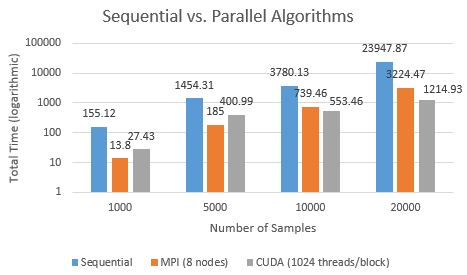
\includegraphics[scale=0.7]{seq_vs_par}
\end{center}
\caption{Logarithmic total time comparison of Sequential and Parallel algorithms against different sized sample sets.}
\label{fig:seq_vs_par}
\end{wrapfigure}

From Figure \ref{fig:seq_vs_par} we can see that the the sequential algorithm's total time is much greater than it's parallel counterparts for all small and large sample sizes.

As both algorithms, sequential and parallel, have $O(n^2)$ complexity, visualizing performance differences with large datasets requires a logarithmic axis.

For smaller sample sizes (less than 5000), the MPI solution outperforms the CUDA solution. This is likely because the root node only needs to broadcast the small input sample vector to each node. As  the sample size gets larger, it must broadcast more samples to each node, and so increasing time taken to do so linearly. 

As the sample size gets larger, in CUDA, the shared memory per block decreases. This results in more kernel warps stalling as their block needs to wait until it's shared memory is ready for the samples it needs. This decreases the kernel's performance. 

For larger sample sizes, CUDA outperforms MPI. This is likely because the amount of MPI node's used is fixed to 8, resulting in more samples per node, while the CUDA implementation can still assign each sample to a unique thread. Section \ref{sect:MPI Node Count} discusses why 8 MPI nodes are used. If a CPU with more resources (cores, threads, and cache) was used, the optimum node count would be greater, resulting in better MPI performance. However, as there are a magnitude more threads available on GPU's, the MPI performance will not out perform the CUDA solution for any large sample sizes.

\section{Further Improvements}\label{sect:improvements}
\subsection{Sub-sample partitioning}
The current algorithmic approach to both MPI and CUDA solutions is to assign output samples to threads and nodes. The downside of this method is that each output sample must act upon all other input samples and is thus sub-quadratic in terms of computational complexity.

A solution to this is to assign a 'master' thread/node to each sample, then assign a unique thread for each input sample. The input sample threads would calculate their real and imaginary parts, which when required by a master thread, would reduce using a custom sum reduction method and then multiply by the input sample.

This solution would require twice as many threads/nodes as samples but would reduce the computation time by having each thread work out a partial solution. The master thread will not be required to calculate real and imaginary parts for all samples; it will just multiply the result from other threads by it's input sample value. The solution will still be of $O(n^2)$ complexity however it's execution time, for each sample, will be reduced linearly.

\subsection{CUDA - Increase Thread-block dimensions}\label{sect:improv_cuda_block}
The current CUDA implementation uses a 1 dimension grid and block layout. Currently, my algorithm is limited to 1024*1024 threads (if assigning 1 thread per sample). As seen in section \ref{sect:Dynamic Shared Memory}, fewer blocks results in higher occupancy, so using 2 or 3 dimension thread blocks will increase our thread and sample limit without increasing the block count. 

This can be done by using a multi-dimensional thread ID lookup code snipped instead of a 1-dimensional thread/block lookup code snipped.

\subsection{CUDA cuDoubleComplex}
My implementation uses 2 double variables, \textit{sum\_real} and \textit{sum\_imag}, to represent the real and imaginary parts of complex numbers.

Using CUDA's built in \textit{cudoubleComplex} type will likely increase performance on a per-instruction basis. CUDA provides built in intrinsic functions for double and complex numbers, like \textit{cuCmul}, that map directly to device instructions.

\section{Conclusion}
From the results in section \ref{sect:seq_vs_par}, it is clear that both parallel CUDA and MPI algorithms exceed the performance of the sequential algorithm for small and large input data sizes. For 20,000 input samples, the sequential implementation takes nearly 24 seconds, while MPI takes 2 seconds and CUDA 1 second, making them more than 10x faster. Even though the sequential implementation requires no memory allocation, it's limited by only being able to operate on a single sample at a time. The CPU and compiler may be optimising the sequential implementation by using SIMD instructions, branch prediction, and other implicit optimisations, but it simply cannot outperform the benefits introduced when using parallel concepts.

The CUDA solution scales better for larger input sample sizes. It's ability to assign a unique thread to each sample makes the algorithm much more efficient in terms of samples per thread. The current implementation is limited to 1024x1024x1 threads/samples, however a slight modification, explained in section \ref{sect:improv_cuda_block}, can increase this limit perhaps to use all available CUDA threads. The use of shared memory in this algorithm was shown to have a negative effect on performance. This is likely an ineffective solution of reducing global memory accesses. The latency introduced by making the 1st thread of each block copy the complete input sample vector to shared memory is not efficient and the results shown in figure \ref{fig:shared_vs_global_graph} show that accessing global memory in the first place was faster than copying the input vector to each block.

Of course, the disadvantage with the CUDA solution is requiring external specific NVIDIA GPU's, which may be size/space (e.g. server racks) constraint and financial constraint. 

As theorized in section \ref{sect:MPI Node Count}, the optimum node count for this algorithm being approximately 2x the number of present CPU cores for small and large data sets. Using a larger CPU with more cores and threads will allow for using more nodes efficiently, reducing the total time. However, the greatest limitation with the MPI solution is the problem of broadcasting the input sample and gathering back the output samples. This becomes a larger problem as the node count increases, even with a more powerful CPU. If using a larger CPU and being able to use more nodes, the problem of communicating between and synchronising the nodes is still a large time demanding problem.

Applying the improvements listed in section \ref{sect:improvements} will benefit the parallel implementations. It will not reduce the complexity of the algorithm from $O(n^2)$ to something closer to the speed of the FFT algorithm, but for large data sets the total time of the algorithm may reduce by multiple seconds.

For one deciding which parallel implementation to use, one must consider their space and financial constraints. The CUDA solution requires an external dedicated GPU which may not be available in server and virtualised environments \citep{server:gpu} and the GPU resources required may require a larger GPU and peripheral investment. In addition, if one's CPU has a low core/thread count, an MPI solution may be bottlenecked by the core/thread count and so off-loading to a GPU may provide a large performance increase.

\newpage
\bibliography{soft354_bib} 

\end{document}
